% !TEX program = pdflatex
\documentclass[aspectratio=169, 11pt]{beamer}

% ── Theme ──
\usetheme{Madrid}
\usecolortheme{seahorse}
\definecolor{DukeBlue}{HTML}{003366}
\definecolor{DukeRoyal}{HTML}{00539B}
\definecolor{WarnRed}{HTML}{CC3333}
\definecolor{OkGreen}{HTML}{2E8B57}
\definecolor{LightGray}{HTML}{F0F0F0}
\setbeamercolor{structure}{fg=DukeBlue}
\setbeamercolor{frametitle}{bg=DukeBlue!10, fg=DukeBlue}
\setbeamercolor{title}{fg=white, bg=DukeBlue}
\setbeamercolor{block title}{bg=DukeBlue!15, fg=DukeBlue}
\setbeamercolor{block body}{bg=DukeBlue!5}
\setbeamercolor{block title alerted}{bg=WarnRed!15, fg=WarnRed}
\setbeamercolor{block body alerted}{bg=WarnRed!5}
\setbeamercolor{block title example}{bg=OkGreen!15, fg=OkGreen!80!black}
\setbeamercolor{block body example}{bg=OkGreen!5}
\setbeamertemplate{navigation symbols}{}
\setbeamertemplate{footline}{%
  \leavevmode\hbox{%
    \begin{beamercolorbox}[wd=.33\paperwidth,ht=2.5ex,dp=1ex,center]{author in head/foot}%
      \usebeamerfont{author in head/foot}\insertshortauthor
    \end{beamercolorbox}%
    \begin{beamercolorbox}[wd=.34\paperwidth,ht=2.5ex,dp=1ex,center]{title in head/foot}%
      \usebeamerfont{title in head/foot}\insertshorttitle
    \end{beamercolorbox}%
    \begin{beamercolorbox}[wd=.33\paperwidth,ht=2.5ex,dp=1ex,right]{date in head/foot}%
      \usebeamerfont{date in head/foot}\insertframenumber{} / \inserttotalframenumber\hspace*{2em}
    \end{beamercolorbox}}%
}

% ── Packages ──
\usepackage[T1]{fontenc}
\usepackage[utf8]{inputenc}
\usepackage{libertine}
\usepackage[libertine]{newtxmath}
\usepackage{inconsolata}
\usepackage{booktabs}
\usepackage{tabularx}
\usepackage{multirow}
\usepackage{array}
\usepackage{amsmath, amssymb}
\usepackage{tikz}
\usetikzlibrary{
  positioning, arrows.meta, calc, backgrounds,
  fit, decorations.pathreplacing, shapes.geometric,
  patterns, shadows, chains
}
\usepackage{pgfplots}
\pgfplotsset{compat=1.18}
\usepackage{xspace}

% ── Macros ──
\newcommand{\mcecog}{$\mu$ECoG\xspace}
\newcommand{\pergood}[1]{\textcolor{OkGreen}{#1}}
\newcommand{\perbad}[1]{\textcolor{WarnRed}{#1}}
\newcommand{\emphcite}[1]{\textcolor{DukeBlue!70}{\footnotesize [#1]}}
\newcolumntype{L}[1]{>{\raggedright\arraybackslash}p{#1}}
\newcolumntype{C}[1]{>{\centering\arraybackslash}p{#1}}

% ── Title ──
\title[Synthetic Pretraining for \mcecog]{%
  Synthetic Grid-Dynamics Pretraining\\for Motor-Speech Decoding from Acute \mcecog}
\author[B.\,Tang]{Ben Tang}
\institute[Cogan Lab]{Cogan Lab, Duke University}
\date{March 2026}

\begin{document}

% ════════════════════════════════════════════════════════
\begin{frame}[plain]
  \titlepage
\end{frame}

% ════════════════════════════════════════════════════════
\begin{frame}{Outline}
  \tableofcontents
\end{frame}

% ════════════════════════════════════════════════════════════
\section{Problem}
% ════════════════════════════════════════════════════════════

\begin{frame}{The Data Bottleneck}

\begin{columns}[T]
\begin{column}{0.55\textwidth}
\textbf{Acute intraoperative \mcecog}:
\begin{itemize}
  \item $\sim$1 min utterance / patient ($\sim$150 trials)
  \item 128--256 channels at 200\,Hz, HGA z-score
  \item 8--12 patients, left sensorimotor cortex
\end{itemize}

\vspace{0.6em}
\textbf{What we know}:
\begin{itemize}
  \item Per-patient CE: \textbf{PER\,=\,0.700} (S14 best)
  \item Cross-patient LOPO: \perbad{PER\,=\,0.846} (near chance)
  \item H=128 backbone: \perbad{55$\times$ train/val gap}
  \item CTC suffers blank collapse (\perbad{95\% blank ratio})
\end{itemize}
\end{column}
\begin{column}{0.42\textwidth}
\begin{block}{Key numbers}
\centering
\small
\begin{tabular}{@{}lr@{}}
  \toprule
  Patients    & 8--12 \\
  Trials/pt   & 46--178 \\
  Sig channels & 63--201 \\
  Phonemes    & 9 (3/trial) \\
  Utterance   & $\sim$1\,min/pt \\
  Total pooled & $\sim$3\,hrs \\
  \bottomrule
\end{tabular}
\end{block}

\vspace{0.5em}
\begin{alertblock}{\small Bottleneck}
  \small Input compression (pool $\to$ 64\,dim) destroys spatial resolution, not GRU capacity.
\end{alertblock}
\end{column}
\end{columns}

\vspace{0.3em}
\emphcite{Spalding 2025; Duraivel 2023, 2025; Singh 2025}
\end{frame}

% ════════════════════════════════════════════════════════════

\begin{frame}{Why Not Existing SSL?}

\begin{columns}[T]
\begin{column}{0.48\textwidth}
\textbf{Spike-based foundation models}\\
{\small BIT (367\,hrs), NDT3 (2000\,hrs)}
\begin{itemize}
  \item Poisson spikes $\neq$ Gaussian HGA
  \item Orders of magnitude more data
\end{itemize}

\vspace{0.6em}
\textbf{ECoG SSL}\\
{\small wav2vec ECoG (CPC, not 2.0)}
\begin{itemize}
  \item Min successful: $\sim$30\,min/pt
  \item We have $\sim$1\,min/pt (30$\times$ smaller)
  \item 1/12 cross-pt transfers worked
\end{itemize}
\end{column}

\begin{column}{0.48\textwidth}
\textbf{What transfers without weights}:
\begin{itemize}
  \item Architecture patterns (TimeSformer, wav2vec)
  \item Masking strategies (VideoMAE)
  \item Per-patient layer design (Singh, Levin)
\end{itemize}

\vspace{0.6em}
\begin{exampleblock}{Opportunity}
  \small Rigid 2D grid structure is \emph{known a priori}---we can synthesize unlimited spatiotemporal movies with controlled inductive biases.
\end{exampleblock}
\end{column}
\end{columns}

\vspace{0.3em}
\emphcite{Zhang 2026 (BIT); wav2vec ECoG; VideoMAE (Tong 2022); Singh 2025; Levin 2026}
\end{frame}

% ════════════════════════════════════════════════════════════
\section{Core Idea}
% ════════════════════════════════════════════════════════════

\begin{frame}{Core Idea: Three-Stage Pipeline}

\begin{center}
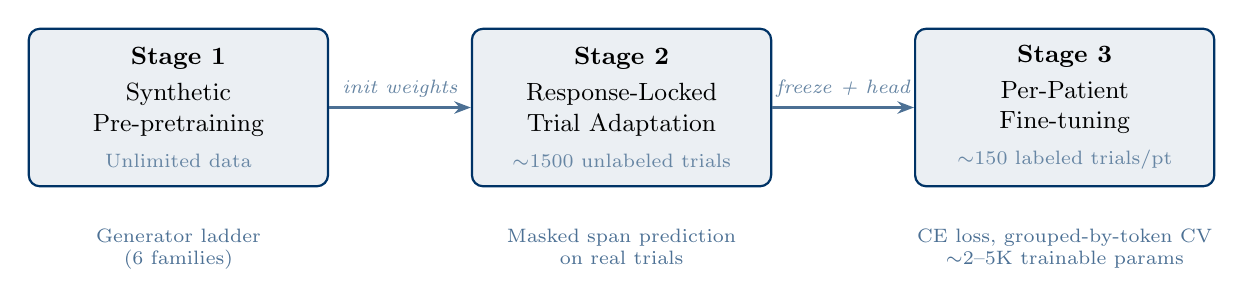
\begin{tikzpicture}[
  stage/.style={
    draw=DukeBlue, thick, rounded corners=4pt,
    minimum width=3.8cm, minimum height=2.0cm,
    fill=DukeBlue!8, align=center, font=\small
  },
  arrow/.style={-{Stealth[length=6pt]}, thick, DukeBlue!70},
  lbl/.style={font=\scriptsize\itshape, text=DukeBlue!60, align=center}
]
  \node[stage] (s1) {%
    \textbf{Stage 1}\\[2pt]
    Synthetic\\Pre-pretraining\\[2pt]
    {\scriptsize\color{DukeBlue!60} Unlimited data}
  };
  \node[stage, right=1.8cm of s1] (s2) {%
    \textbf{Stage 2}\\[2pt]
    Response-Locked\\Trial Adaptation\\[2pt]
    {\scriptsize\color{DukeBlue!60} $\sim$1500 unlabeled trials}
  };
  \node[stage, right=1.8cm of s2] (s3) {%
    \textbf{Stage 3}\\[2pt]
    Per-Patient\\Fine-tuning\\[2pt]
    {\scriptsize\color{DukeBlue!60} $\sim$150 labeled trials/pt}
  };

  \draw[arrow] (s1) -- node[above, lbl] {init weights} (s2);
  \draw[arrow] (s2) -- node[above, lbl] {freeze + head} (s3);

  % data labels below
  \node[below=0.4cm of s1, font=\scriptsize, align=center, text=DukeBlue!70] {%
    Generator ladder\\(6 families)};
  \node[below=0.4cm of s2, font=\scriptsize, align=center, text=DukeBlue!70] {%
    Masked span prediction\\on real trials};
  \node[below=0.4cm of s3, font=\scriptsize, align=center, text=DukeBlue!70] {%
    CE loss, grouped-by-token CV\\$\sim$2--5K trainable params};
\end{tikzpicture}
\end{center}

\vspace{0.5em}

\begin{columns}[T]
\begin{column}{0.48\textwidth}
\textbf{Hypothesis}: Synthetic spatiotemporal dynamics teach an encoder to process 2D grids evolving over time. This transfers to real cortical activity.
\end{column}
\begin{column}{0.48\textwidth}
\textbf{Analogy}: Both synthetic generators and \mcecog produce 2D grids evolving over time; the model must extract spatial patterns and track temporal evolution.
\end{column}
\end{columns}
\end{frame}

% ════════════════════════════════════════════════════════════

\begin{frame}{Three Claims}

\begin{enumerate}
\item \textbf{Does SSL pretraining help} for acute intra-op \mcecog motor-speech decoding at $<$200 trials/patient?
  \begin{itemize}
    \item[\scriptsize$\triangleright$] \small Test: Method A/B vs D (supervised baseline)
  \end{itemize}

\vspace{0.4em}
\item \textbf{Does synthetic pre-pretraining add value} beyond real-data-only SSL?
  \begin{itemize}
    \item[\scriptsize$\triangleright$] \small Test: Method A vs B (neural-only); Method J controls for step count
  \end{itemize}

\vspace{0.4em}
\item \textbf{Does structured synthetic dynamics help} beyond matched-statistics non-dynamic exposure?
  \begin{itemize}
    \item[\scriptsize$\triangleright$] \small Test: Method A vs K (destroyed-dynamics control)
  \end{itemize}
\end{enumerate}

\vspace{0.8em}
\begin{block}{Primary endpoint}
  Full-window readout $[-0.5, +1.0\text{s}]$ with per-position CE---validated at PER\,=\,0.700.\\
  Motor-focused $[-0.15, +0.6\text{s}]$ is preregistered mechanistic secondary.
\end{block}
\end{frame}

% ════════════════════════════════════════════════════════════
\section{Stage 1: Synthetic Pre-pretraining}
% ════════════════════════════════════════════════════════════

\begin{frame}{Generator Ladder: Comparative Hierarchy}

\centering
\footnotesize
\renewcommand{\arraystretch}{1.05}
\begin{tabular}{@{}c l c c c L{4.0cm}@{}}
  \toprule
  \textbf{Lv} & \textbf{Generator} & \rotatebox{70}{\scriptsize\textbf{Local coup.}} & \rotatebox{70}{\scriptsize\textbf{Nonlinear}} & \rotatebox{70}{\scriptsize\textbf{Diverse}} & \textbf{New property} \\
  \midrule
  0 & Smooth Gaussian AR & & & & \textit{Baseline}: smooth, correlated \\
  1 & Switching LDS       & \checkmark & & & Regime switching \\
  2 & Damped Wave          & \checkmark & & & Oscillatory local coupling \\
  3 & Gray--Scott          & \checkmark & \checkmark & & Nonlinearity (RD) \\
  4 & FitzHugh--Nagumo     & \checkmark & \checkmark & & Excitable-medium dynamics \\
  5 & NCA Random MLP       & \checkmark & \checkmark & \checkmark & Rule diversity \\
  \bottomrule
\end{tabular}

\vspace{0.5em}

\begin{columns}[T]
\begin{column}{0.48\textwidth}
\small
\textbf{Key comparisons}:
\begin{itemize}\setlength{\itemsep}{0pt}
  \item L0 vs L1: regime switching?
  \item L1 vs L2: oscillatory coupling?
  \item L2 vs L3--4: nonlinearity?
  \item L4 vs L5: rule diversity?
  \item L0 vs Mixed: everything together?
\end{itemize}
\end{column}
\begin{column}{0.48\textwidth}
\small
\textbf{If Mixed wins}, the paper becomes ``diverse synthetic dynamics help''---not ``cortex-like dynamics help.'' Both interpretations prepared.

\vspace{0.3em}
\textbf{Also}: Sequential hotspot activation (Gaussian bump on random trajectory) tests trajectory vs.\ local-coupling structure.
\end{column}
\end{columns}

\vspace{0.2em}
\emphcite{Lee et al.\ 2026 (NCA); Ghahramani \& Hinton 2000 (switching LDS)}
\end{frame}

% ════════════════════════════════════════════════════════════

\begin{frame}{Generator Ladder: Confounds \& Calibration}

\begin{alertblock}{Confound acknowledgment}
\small
Each level changes a primary property \emph{and} secondary characteristics (spectral shape, stationarity, event morphology). If L3\,$>$\,L2, nonlinearity is \emph{associated} with improvement, not strictly causal---Gray--Scott also changes spectral shape relative to the damped wave. Pairwise matched controls deferred. \textbf{Method K} provides an orthogonal cut: dynamics vs.\ statistics.
\end{alertblock}

\vspace{0.4em}

\begin{columns}[T]
\begin{column}{0.48\textwidth}
\begin{block}{\small Coarse calibration (source-only)}
\scriptsize
1--2 params/generator to avoid degenerate dynamics:
\begin{itemize}\setlength{\itemsep}{0pt}
  \item PSD: main power below 20\,Hz
  \item Spatial correlation: 2--10 electrodes
  \item Kurtosis $> 2$
  \item Event sparsity: 5--30\%
\end{itemize}
Not optimization---prevents blowup/collapse.
\end{block}
\end{column}
\begin{column}{0.48\textwidth}
\begin{block}{\small Matching statistics (source pts only)}
\scriptsize
Computed for each generator vs real uECOG:
\begin{itemize}\setlength{\itemsep}{0pt}
  \item Temporal PSD (Welch, evoked + residual)
  \item Spatial covariance length scale
  \item Amplitude distribution (kurtosis)
  \item Dead-mask prevalence
  \item Event sparsity per trial phase
  \item RT distribution (log-normal fit)
\end{itemize}
\end{block}
\end{column}
\end{columns}
\end{frame}

% ════════════════════════════════════════════════════════════

\begin{frame}{Synthetic Trial Anatomy}

\begin{center}
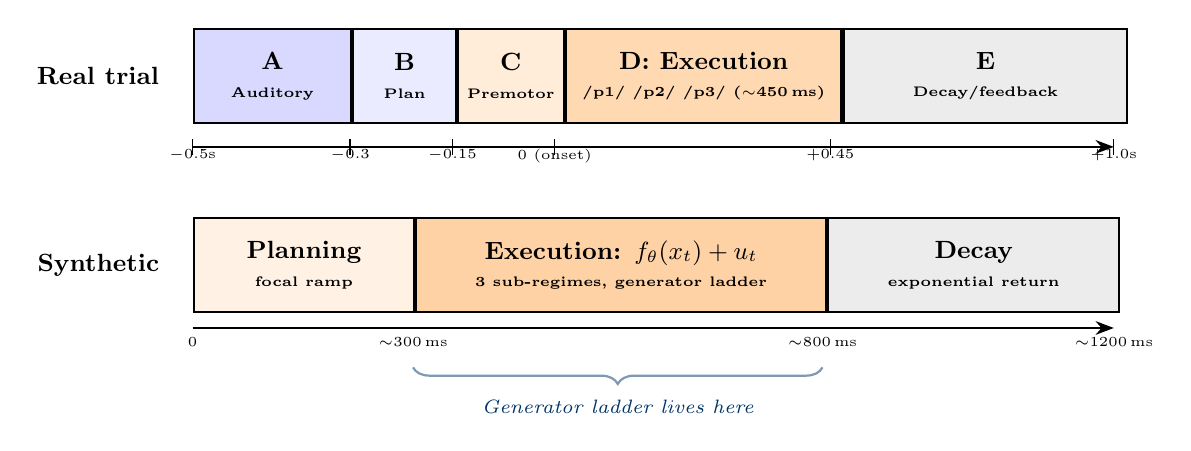
\begin{tikzpicture}[
  xscale=1.0,
  phase/.style={draw, thick, minimum height=1.2cm, anchor=west, font=\small\bfseries, align=center},
]
  % Real trial
  \node[font=\small\bfseries, anchor=east] at (-0.3, 2.4) {Real trial};

  \node[phase, fill=blue!15, minimum width=2.0cm] (rA) at (0, 2.4) {A\\[-1pt]{\tiny Auditory}};
  \node[phase, fill=blue!8, minimum width=1.3cm, right=0pt of rA] (rB) {B\\[-1pt]{\tiny Plan}};
  \node[phase, fill=orange!15, minimum width=1.3cm, right=0pt of rB] (rC) {C\\[-1pt]{\tiny Premotor}};
  \node[phase, fill=orange!30, minimum width=3.5cm, right=0pt of rC] (rD) {D: Execution\\[-1pt]{\tiny /p1/ /p2/ /p3/ ($\sim$450\,ms)}};
  \node[phase, fill=gray!15, minimum width=3.6cm, right=0pt of rD] (rE) {E\\[-1pt]{\tiny Decay/feedback}};

  \draw[thick, -{Stealth}] (0, 1.5) -- (11.7, 1.5);
  \foreach \x/\t in {0/$-$0.5s, 2.0/$-$0.3, 3.3/$-$0.15, 4.6/0 (onset), 8.1/+0.45, 11.7/+1.0s} {
    \draw (\x, 1.4) -- (\x, 1.6) node[below, font=\tiny] {\t};
  }

  % Synthetic trial
  \node[font=\small\bfseries, anchor=east] at (-0.3, 0) {Synthetic};

  \node[phase, fill=orange!10, minimum width=2.8cm] (sP) at (0, 0) {Planning\\[-1pt]{\tiny focal ramp}};
  \node[phase, fill=orange!35, minimum width=5.2cm, right=0pt of sP] (sE) {Execution: $f_\theta(x_t) + u_t$\\[-1pt]{\tiny 3 sub-regimes, generator ladder}};
  \node[phase, fill=gray!15, minimum width=3.7cm, right=0pt of sE] (sD) {Decay\\[-1pt]{\tiny exponential return}};

  \draw[thick, -{Stealth}] (0, -0.8) -- (11.7, -0.8);
  \node[below, font=\tiny] at (0, -0.8) {0};
  \node[below, font=\tiny] at (2.8, -0.8) {$\sim$300\,ms};
  \node[below, font=\tiny] at (8.0, -0.8) {$\sim$800\,ms};
  \node[below, font=\tiny] at (11.7, -0.8) {$\sim$1200\,ms};

  % Annotation
  \draw[decorate, decoration={brace, amplitude=6pt, mirror}, thick, DukeBlue!50]
    (2.8, -1.3) -- (8.0, -1.3) node[midway, below=8pt, font=\scriptsize\itshape, text=DukeBlue] {%
      Generator ladder lives here};
\end{tikzpicture}
\end{center}

\vspace{0.3em}
\small
\textbf{Forced generators}: $x_{t+1} = f_\theta(x_t) + u_t$ where $u_t$ is phase-dependent drive.
Sub-event templates are \emph{generic} random focal patterns, NOT phoneme-specific.

\vspace{0.2em}
\textbf{Nuisance realism}: z-normalize $\to$ IID noise ($\sigma \sim \mathcal{U}(0.3, 0.8)$) $\to$ correlated noise (rank 1--3, SD $\sim \mathcal{U}(0.2, 0.6)$) $\to$ dead electrode masks $\to$ anti-alias LPF $\to$ subsample to 20\,Hz.
\end{frame}

% ════════════════════════════════════════════════════════════

\begin{frame}{Masking Objective}

\begin{columns}[T]
\begin{column}{0.55\textwidth}

\textbf{Masked temporal span prediction}:
\begin{enumerate}
  \item Mask 40--60\% of frames (3--6 spans)
  \item Predict masked frames from bidirectional context
  \item Loss = MSE(predicted, actual) on masked frames only
\end{enumerate}

\vspace{0.4em}
\textbf{Why aggressive masking?}\\
{\small At 20\,Hz (30 frames/trial), the signal is smooth and temporally autocorrelated. 10--17\% masking $\to$ trivially solvable by linear interpolation.}

\vspace{0.4em}
\emphcite{VideoMAE (Tong 2022): aggressive masking critical for SSL on smooth signals}

\end{column}
\begin{column}{0.42\textwidth}

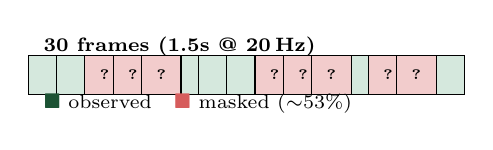
\begin{tikzpicture}[scale=0.6]
  % Observed frames
  \foreach \i in {0,1,5,6,7,11,14} {
    \node[draw, fill=OkGreen!20, minimum size=0.5cm, inner sep=0pt, font=\tiny]
      at (\i*0.6, 0) {};
  }
  % Masked frames
  \foreach \i in {2,3,4,8,9,10,12,13} {
    \node[draw, fill=WarnRed!25, minimum size=0.5cm, inner sep=0pt, font=\tiny]
      at (\i*0.6, 0) {\textbf{?}};
  }
  \node[font=\scriptsize, anchor=west] at (-0.3, -0.6) {%
    \textcolor{OkGreen!60!black}{$\blacksquare$} observed\quad
    \textcolor{WarnRed!80}{$\blacksquare$} masked ($\sim$53\%)};
  \node[font=\scriptsize\bfseries, anchor=west] at (-0.3, 0.6) {30 frames (1.5s @ 20\,Hz)};
\end{tikzpicture}

\vspace{0.6em}
\begin{block}{\small Required baselines}
\scriptsize
\begin{enumerate}
  \item Linear interpolation
  \item Phase-template average
  \item Patient-specific template
  \item Cropped-window eval
  \item Destroyed-dynamics (Method K)
\end{enumerate}
\end{block}
\end{column}
\end{columns}
\end{frame}

% ════════════════════════════════════════════════════════════
\section{Stage 2: Trial Adaptation}
% ════════════════════════════════════════════════════════════

\begin{frame}{Stage 2: Response-Locked Trial Adaptation}

\begin{alertblock}{Honest supervision accounting}
\small
Stage 2 uses \textbf{no phoneme labels} but is \textbf{not unsupervised}. It requires response-onset timestamps (MFA), trial identity (every sample is a speech trial), and patient identity. This is \textbf{weakly-supervised trial-epoch adaptation}.
\end{alertblock}

\vspace{0.2em}
\small
\textbf{The shortcut problem}: Response-locked trials have a stereotyped phase calendar (auditory $\to$ plan $\to$ execute $\to$ decay). The acoustic regression pivot showed 500ms-shifted controls were competitive---the model learned trial structure, not phoneme-sensitive mappings.

\vspace{0.3em}
\textbf{Anti-leakage defenses}:

\begin{columns}[T]
\begin{column}{0.48\textwidth}
\begin{exampleblock}{\small 1. Full-epoch off-center crops}
\scriptsize
Load $[-1.0, 1.5\text{s}]$ (50 frames @ 20\,Hz).\\
Crop to 30--40 frames with random offset.\\
\textbf{Removes entire phases} from some samples.
\end{exampleblock}
\end{column}
\begin{column}{0.48\textwidth}
\begin{exampleblock}{\small 2. Time-reversal augmentation}
\scriptsize
10\% probability: reverse temporal order.\\
Destroys causal phase ordering.\\
If it hurts $\to$ model relies on phase structure.
\end{exampleblock}
\end{column}
\end{columns}

\vspace{0.2em}
\small\textbf{Transfer-proxy gate}: Probe every 5K steps on locked dev patient. Earliest-within-1SE checkpoint rule. Source-only sensitivity analysis alongside.
\end{frame}

% ════════════════════════════════════════════════════════════

\begin{frame}{Stage 2: Patient Pools \& Diagnostics}

\centering
\small
\renewcommand{\arraystretch}{1.15}
\begin{tabular}{@{}l L{3.4cm} L{4.2cm} L{2.5cm}@{}}
  \toprule
  \textbf{Mode} & \textbf{Synth calibration} & \textbf{Stage 2 neural pool} & \textbf{Evaluation} \\
  \midrule
  \textbf{Inductive} (primary) & PS $\setminus \{d, t\}$ & Unlabeled trials: PS $\setminus \{d, t\}$ & Patient $t$ \\
  \textbf{Transductive} (secondary) & Same as inductive & Unlabeled trials: PS $\setminus \{d\}$ (incl.\ $t$) & Patient $t$ \\
  \bottomrule
\end{tabular}

\vspace{0.3em}
{\footnotesize $d$ = fixed dev patient (e.g., S26), $t$ = target patient in current fold.}

\vspace{0.8em}

\begin{columns}[T]
\begin{column}{0.48\textwidth}
\begin{block}{\small Required diagnostics}
\small
\begin{itemize}
  \item Per-phase prediction loss
  \item Patient-ID vs phoneme-ID probes
  \item Content-collapse check:
    \begin{itemize}\scriptsize
      \item Output entropy $< 1.5$ bits $\to$ alarm
      \item Unigram KL from uniform
      \item Stereotypy index $< 10\%$ $\to$ alarm
    \end{itemize}
\end{itemize}
\end{block}
\end{column}
\begin{column}{0.48\textwidth}
\begin{block}{\small JEPA escalation triggers}
\small
Promote latent prediction if \textbf{any} of:
\begin{enumerate}\small
  \item Event-frame gains vanish at execution-only decoding
  \item Patient-ID $> 2\sigma$ without phoneme-ID gain
  \item Pretext MSE plateaus $>$5K steps w/o transfer-proxy lift
\end{enumerate}
\end{block}
\end{column}
\end{columns}

\emphcite{JEPA: Assran et al.\ 2023 (I-JEPA)}
\end{frame}

% ════════════════════════════════════════════════════════════
\section{Architecture}
% ════════════════════════════════════════════════════════════

\begin{frame}{Three Architecture Families}

\begin{center}
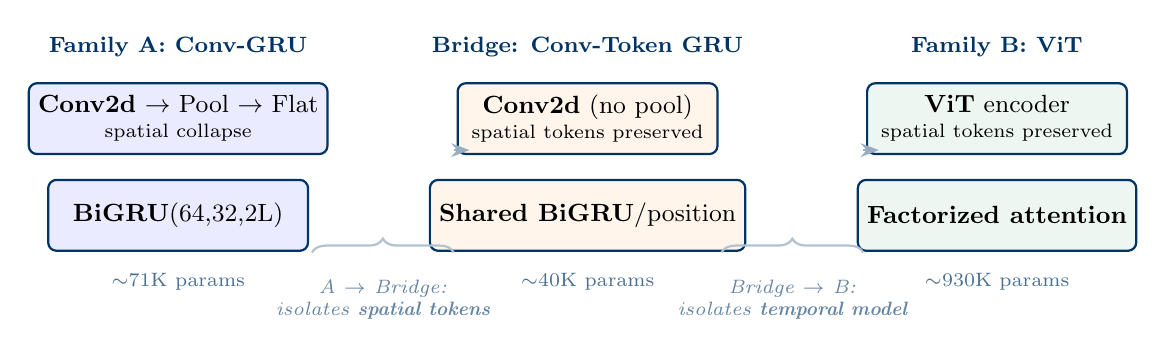
\begin{tikzpicture}[
  box/.style={draw=DukeBlue, thick, rounded corners=3pt, minimum height=0.9cm,
    minimum width=3.0cm, fill=#1, align=center, font=\small},
  box/.default={DukeBlue!8},
  lbl/.style={font=\scriptsize, text=DukeBlue!70},
  >=Stealth
]

% Family A
\node[box=blue!8, minimum width=3.3cm] (a_enc) at (0, 0)
  {\textbf{Conv2d} $\to$ Pool $\to$ Flat\\[-2pt]{\scriptsize spatial collapse}};
\node[box=blue!8, minimum width=3.3cm, below=0.3cm of a_enc] (a_pred)
  {\textbf{BiGRU}(64,32,2L)};
\node[font=\footnotesize\bfseries, above=0.2cm of a_enc, text=DukeBlue] {Family A: Conv-GRU};
\node[lbl, below=0.15cm of a_pred] {$\sim$71K params};

% Conv-token GRU
\node[box=orange!8, minimum width=3.3cm] (ct_enc) at (5.2, 0)
  {\textbf{Conv2d} (no pool)\\[-2pt]{\scriptsize spatial tokens preserved}};
\node[box=orange!8, minimum width=3.3cm, below=0.3cm of ct_enc] (ct_pred)
  {\textbf{Shared BiGRU}/position};
\node[font=\footnotesize\bfseries, above=0.2cm of ct_enc, text=DukeBlue] {Bridge: Conv-Token GRU};
\node[lbl, below=0.15cm of ct_pred] {$\sim$40K params};

% Family B
\node[box=OkGreen!8, minimum width=3.3cm] (b_enc) at (10.4, 0)
  {\textbf{ViT} encoder\\[-2pt]{\scriptsize spatial tokens preserved}};
\node[box=OkGreen!8, minimum width=3.3cm, below=0.3cm of b_enc] (b_pred)
  {\textbf{Factorized attention}};
\node[font=\footnotesize\bfseries, above=0.2cm of b_enc, text=DukeBlue] {Family B: ViT};
\node[lbl, below=0.15cm of b_pred] {$\sim$930K params};

% Arrows between families
\draw[thick, DukeBlue!40, -{Stealth}, dashed] (3.5, -0.4) -- (3.7, -0.4)
  node[midway, above, font=\tiny, text=DukeBlue!60] {};
\draw[thick, DukeBlue!40, -{Stealth}, dashed] (8.7, -0.4) -- (8.9, -0.4);

% Comparison annotations
\node[font=\scriptsize\itshape, text=DukeBlue!60, align=center] at (2.6, -2.3)
  {A $\to$ Bridge:\\isolates \textbf{spatial tokens}};
\node[font=\scriptsize\itshape, text=DukeBlue!60, align=center] at (7.8, -2.3)
  {Bridge $\to$ B:\\isolates \textbf{temporal model}};

\draw[thick, DukeBlue!30, decorate, decoration={brace, amplitude=5pt}]
  (1.7, -1.7) -- (3.5, -1.7);
\draw[thick, DukeBlue!30, decorate, decoration={brace, amplitude=5pt}]
  (6.9, -1.7) -- (8.7, -1.7);

\end{tikzpicture}
\end{center}

\vspace{0.3em}

\begin{columns}[T]
\begin{column}{0.32\textwidth}
\small
\textbf{Conv-GRU} (conservative):\\
Preserves spatial-collapse bottleneck. If pretraining helps \emph{despite} this $\to$ robust signal.
\end{column}
\begin{column}{0.32\textwidth}
\small
\textbf{Conv-Token GRU} (bridge):\\
Per-position BiGRU, no cross-position interaction. Isolates spatial preservation.
\end{column}
\begin{column}{0.32\textwidth}
\small
\textbf{ViT} (high-capacity):\\
Factorized space-time attention. Freezing required ($\sim$5.3K trainable at Stage~3).
\end{column}
\end{columns}

\emphcite{TimeSformer (Bertasius 2021); Singh 2025 (per-patient layers)}
\end{frame}

% ════════════════════════════════════════════════════════════

\begin{frame}{Spatial Pooling \& Positional Encoding}

\begin{columns}[T]
\begin{column}{0.48\textwidth}
\textbf{Spatial pooling} (Family B \& Bridge):
\begin{itemize}
  \item \textbf{Mean-pool} (co-default): simple average
  \item \textbf{Top-$k$ pool} (co-default, $k$=16): average $k$ highest-norm tokens. Parameter-free
  \item \textbf{Learned attention} (Tier 1 ablation): query cross-attends to spatial tokens, +33K params
\end{itemize}

\vspace{0.3em}
\small\textit{Rationale}: Mean-pool erases focal articulatory activation on $<$2mm grids. Top-$k$ is the parameter-free fix.

\end{column}
\begin{column}{0.48\textwidth}
\textbf{Positional encoding}:

\begin{block}{\small Local geometry PE (default)}
\small
$\text{PE} = \text{Linear}(3 \to d)$ on:\\
\quad (row $\times$ pitch\textsubscript{mm},\; col $\times$ pitch\textsubscript{mm},\; dead\_frac)\\[4pt]
Known pitches: 128ch = 1.33\,mm, 256ch 12$\times$22 = 1.72\,mm.\\
8$\times$32/8$\times$34: surrogate 1.33\,mm (flagged).
\end{block}

\vspace{0.3em}
\small
\textbf{Not included}: MNI anatomical encoding (future ablation---local mm coordinates do NOT encode where the array sits on cortex).

\vspace{0.2em}
\textbf{Augmentation consistency}: Flips/rotations must transform PE inputs identically.
\end{column}
\end{columns}
\end{frame}

% ════════════════════════════════════════════════════════════
\section{Experimental Design}
% ════════════════════════════════════════════════════════════

\begin{frame}{Comparison Methods (First Round)}

\centering
\small
\renewcommand{\arraystretch}{1.15}
\begin{tabular}{@{}c l L{7.5cm} c@{}}
  \toprule
  & \textbf{Method} & \textbf{Description} & \textbf{Tests} \\
  \midrule
  A & Structured Synth + Neural & Mixed pool \{switching LDS, wave, GS, FHN, NCA, hotspot\} $\to$ neural & Hypothesis \\
  B & Neural Only & Masked span on real trials, random init & Claim 1 \\
  C & Smooth AR + Neural & Generic smooth synthetic $\to$ neural & Claim 2 \\
  D & Supervised Baseline & No pretraining, end-to-end CE & Baseline \\
  E & Random-Init Frozen & Freeze random encoder, train head only & Noise floor \\
  F & Random-Scaffold + Neural & Same generators, random phase count & Scaffold \\
  K & Destroyed-Dynamics + Neural & Phase-randomized / time-shuffled & \textbf{Claim 3} \\
  \midrule
  J & B-Extended ($2\times$ steps) & \multicolumn{2}{l}{\textit{Automatic if A\,$>$\,B by bootstrap CI}} \\
  \bottomrule
\end{tabular}

\vspace{0.5em}
\textbf{Step-matched}: A, B, C, F, K all get $S_\text{total}$ optimizer steps.\\
\textbf{Residual confound}: A sees unlimited synthetic diversity; B reuses $\sim$1500 trials. Method J controls this.
\end{frame}

% ════════════════════════════════════════════════════════════

\begin{frame}{Execution Order: Pilot-First Sequencing}

\begin{center}
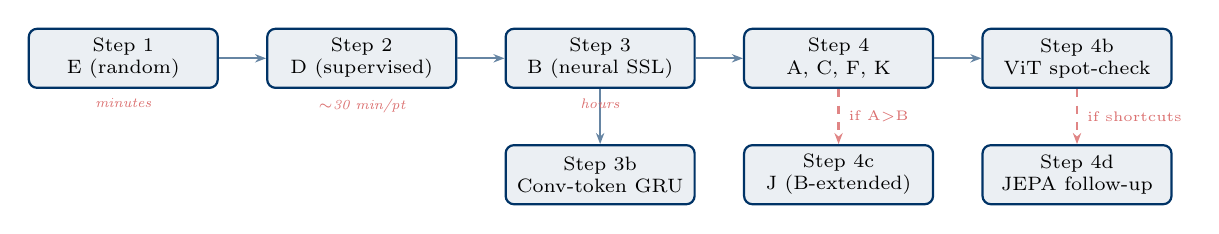
\begin{tikzpicture}[
  sbox/.style={draw=DukeBlue, thick, rounded corners=3pt,
    minimum width=2.4cm, minimum height=0.75cm,
    fill=DukeBlue!8, align=center, font=\scriptsize},
  gate/.style={draw=WarnRed!80, thick, rounded corners=3pt, diamond,
    aspect=2.5, fill=WarnRed!8, font=\scriptsize, inner sep=2pt},
  arr/.style={-{Stealth[length=4pt]}, thick, DukeBlue!60},
  garr/.style={-{Stealth[length=4pt]}, thick, WarnRed!60, dashed},
]
  \node[sbox] (e) at (0, 0) {Step 1\\E (random)};
  \node[sbox, right=0.6cm of e] (d) {Step 2\\D (supervised)};
  \node[sbox, right=0.6cm of d] (b) {Step 3\\B (neural SSL)};
  \node[sbox, right=0.6cm of b] (acfk) {Step 4\\A, C, F, K};
  \node[sbox, right=0.6cm of acfk] (vit) {Step 4b\\ViT spot-check};

  \node[sbox, below=0.7cm of b] (ct) {Step 3b\\Conv-token GRU};
  \node[sbox, below=0.7cm of acfk] (j) {Step 4c\\J (B-extended)};
  \node[sbox, below=0.7cm of vit] (jepa) {Step 4d\\JEPA follow-up};

  \draw[arr] (e) -- (d);
  \draw[arr] (d) -- (b);
  \draw[arr] (b) -- (acfk);
  \draw[arr] (acfk) -- (vit);

  \draw[arr] (b.south) -- (ct.north);
  \draw[garr] (acfk.south) -- node[right, font=\tiny, text=WarnRed!70] {if A$>$B} (j.north);
  \draw[garr] (vit.south) -- node[right, font=\tiny, text=WarnRed!70] {if shortcuts} (jepa.north);

  % Gates
  \node[font=\tiny\itshape, text=WarnRed!70, below=0pt of e] {minutes};
  \node[font=\tiny\itshape, text=WarnRed!70, below=0pt of d] {$\sim$30 min/pt};
  \node[font=\tiny\itshape, text=WarnRed!70, below=0pt of b] {hours};
\end{tikzpicture}
\end{center}

\vspace{0.3em}
\small
\textbf{Interpretation ladder} (Step 4):
\begin{center}
\scriptsize
\renewcommand{\arraystretch}{1.1}
\begin{tabular}{@{}l l@{}}
  \toprule
  \textbf{Outcome} & \textbf{Interpretation} \\
  \midrule
  $\text{A} > \text{K} > \text{C} > \text{B}$ & Structured dynamics help beyond statistics (\textbf{strongest}) \\
  $\text{A} > \text{F} > \text{C} > \text{B}$ & 3-event scaffold matters \\
  $\text{A} \approx \text{K} > \text{C} > \text{B}$ & Spatial statistics help, not dynamics (narrower claim) \\
  $\text{A} \approx \text{C} > \text{B}$ & Any smooth pretraining helps (weakest publishable) \\
  $\text{A} \approx \text{B} \approx \text{D}$ & SSL doesn't help (null result) \\
  \bottomrule
\end{tabular}
\end{center}
\end{frame}

% ════════════════════════════════════════════════════════════
\section{Stage 3 \& Evaluation}
% ════════════════════════════════════════════════════════════

\begin{frame}{Stage 3: Per-Patient Fine-tuning}

\begin{columns}[T]
\begin{column}{0.48\textwidth}
\textbf{Default freeze configuration}:\\
Freeze all except:
\begin{itemize}
  \item CE classification head
  \item Per-patient Conv2d / patch embed
  \item Predictor LayerNorm parameters
\end{itemize}

\vspace{0.2em}
\small
Trainable: $\sim$2.3K (conv-GRU), $\sim$2.2K (bridge), $\sim$5.3K (ViT)

\vspace{0.5em}
\textbf{Cross-validation}:\\
Grouped-by-token (all reps of same CVC/VCV token in same fold). Fixed splits saved to JSON, reused across all methods.

\vspace{0.2em}
{\footnotesize\itshape Note: 0.700 PER used stratified CV---not directly comparable.}
\end{column}

\begin{column}{0.48\textwidth}
\textbf{Readout windows}:
\begin{enumerate}
  \item \textbf{Full-window} $[-0.5, +1.0\text{s}]$\\
    {\small headline primary, validated at PER\,=\,0.700}
  \item \textbf{Motor-focused} $[-0.15, +0.6\text{s}]$\\
    {\small preregistered mechanistic secondary}
  \item \textbf{Execution-only} $[0, +0.5\text{s}]$\\
    {\small ablation, strictest test}
\end{enumerate}

\vspace{0.4em}
\textbf{Loss}: 27-way CE (3 pos $\times$ 9 phonemes)\\
+ Three-bin temporal pooling (secondary)

\vspace{0.4em}
\begin{block}{\small Content-collapse checks}
\scriptsize
Entropy, unigram KL, stereotypy index.\\
LOPO CE showed 100\% correct-length but only 21\% position accuracy.
\end{block}
\end{column}
\end{columns}
\end{frame}

% ════════════════════════════════════════════════════════════

\begin{frame}{Statistical Framework}

\begin{columns}[T]
\begin{column}{0.50\textwidth}
\small
\textbf{Patient-level aggregation}:\\
Atomic unit = mean PER across CV folds per patient per method.

\vspace{0.3em}
\textbf{Population statistics}:
\begin{itemize}\setlength{\itemsep}{0pt}
  \item Per-patient table (all methods, all windows)
  \item Mean $\pm$ std of patient-level PER
  \item \textbf{Wilcoxon signed-rank} on paired PERs
  \item Bootstrap 95\% CIs (10K resamples)
  \item Cohen's $d$ + Holm--Bonferroni correction
\end{itemize}

\vspace{0.2em}
\textbf{Primary}: A vs D, A vs B\\
\textbf{Secondary}: A vs C, A vs F, A vs K
\end{column}

\begin{column}{0.46\textwidth}
\begin{block}{\small Surrogate null control}
\small
For A vs D headline: permute phoneme labels within each patient (preserving patient/fold structure), retrain Stage 3 head, compute PER. 100$\times$ per patient.\\[4pt]
If real improvement falls within null 95th percentile $\to$ gain is not label-informative.
\end{block}

\vspace{0.4em}
\begin{exampleblock}{\small Power considerations}
\small
$N = 8$--$12$ patients with noisy estimates. Bootstrap CIs + per-patient scatter plots + effect sizes supplement Wilcoxon.
\end{exampleblock}
\end{column}
\end{columns}
\end{frame}

% ════════════════════════════════════════════════════════════
\section{Risks \& Mitigations}
% ════════════════════════════════════════════════════════════

\begin{frame}{Known Risks \& Defenses}

\footnotesize
\renewcommand{\arraystretch}{1.15}
\begin{tabular}{@{}L{3.0cm} L{5.2cm} L{4.5cm}@{}}
  \toprule
  \textbf{Risk} & \textbf{Mitigation} & \textbf{Evidence / Precedent} \\
  \midrule
  Synth $\to$ neural gap & Nuisance aug, coarse calibration, Method C/K & VideoMAE, I-JEPA: gap bridgeable \\
  Trivial interpolation & 40--60\% masking, interp.\ baseline, event-frame diagnostic & VideoMAE: smooth signals need aggressive masking \\
  Trial-calendar leakage & Off-center crops, time-reversal aug, per-phase loss & Acoustic regression: 500ms-shift competitive \\
  Content collapse & Entropy/KL/stereotypy diagnostics & LOPO: 95\% blank (CTC), 21\% acc (CE) \\
  ViT overfitting & Freeze all but $\sim$5.3K; conv-GRU fallback & H=128: 55$\times$ train/val gap \\
  Low power ($N$=8--12) & Bootstrap CIs, surrogate null, per-patient plots & Standard for intra-op BCI \\
  \bottomrule
\end{tabular}

\vspace{0.4em}
\small
\textbf{Precautionary lessons}: Data scarcity is the wall $\cdot$ Per-patient adaptation is the default assumption \emphcite{Singh 2025} $\cdot$ Auxiliary targets need negative controls $\cdot$ MPS breaks with mixed grid sizes.
\end{frame}

% ════════════════════════════════════════════════════════════
\section{Decisions for This Meeting}
% ════════════════════════════════════════════════════════════

\begin{frame}{Decisions to Lock}

\begin{enumerate}
\item \textbf{Headline evaluation contract}:\\
  {\small Inductive Stage 2 primary $\cdot$ Full-window CE primary endpoint $\cdot$ Motor-focused secondary}

\vspace{0.3em}
\item \textbf{First-round architecture set}:\\
  {\small Conv-GRU pilot $\to$ conv-token GRU bridge $\to$ ViT spot-check with paired adapter ablation}

\vspace{0.3em}
\item \textbf{Stage 2 interpretation language}:\\
  {\small ``Weakly supervised response-locked trial adaptation'' (not ``unsupervised neural SSL'')}

\vspace{0.3em}
\item \textbf{Surrogate-pitch fallback}:\\
  {\small 1.33\,mm for 8$\times$32/8$\times$34 until hardware specs verified?}

\vspace{0.3em}
\item \textbf{Dev patient selection}:\\
  {\small Single fixed dev patient (e.g., S26: 151 trials, 8$\times$16, 74 sig ch)? Or different rule?}
\end{enumerate}

\vspace{0.5em}
\textbf{Meeting output}: Locked claim language, first-round method list, implementation order, verification tasks.
\end{frame}

% ════════════════════════════════════════════════════════════

\begin{frame}{Open Questions}

\begin{columns}[T]
\begin{column}{0.48\textwidth}
\textbf{Design questions}:
\begin{enumerate}\small
  \item Masked spans vs causal multi-step? {\scriptsize(default: spans)}
  \item FHN parameter ranges---map interesting regime
  \item Multi-variable observation for FHN: $(H,W,2)$ or $(H,W,1)$?
  \item Prediction target space: raw patches or encoder tokens (stop-grad)?
  \item Predictor depth: 2 vs 4 layers?
\end{enumerate}
\end{column}
\begin{column}{0.48\textwidth}
\textbf{External verification}:
\begin{enumerate}\setcounter{enumi}{5}\small
  \item \textbf{Array pitch} for 8$\times$32 and 8$\times$34---confirm from hardware docs or Zac
  \item \textbf{Dev patient}: S26? Confirm
  \item \textbf{Motor-focused crop}: exact boundaries from per-patient MFA timing? Patient-specific vs fixed?
\end{enumerate}

\vspace{0.4em}
\begin{block}{\small Implementation order}
\scriptsize
\begin{enumerate}
  \item Protocol scaffolding
  \item Stage 1 synthetic stack
  \item Model stack
  \item Stage 2 training
  \item Stage 3 evaluation
  \item First-round execution
  \item JEPA follow-up gate
\end{enumerate}
\end{block}
\end{column}
\end{columns}
\end{frame}

% ════════════════════════════════════════════════════════════

\begin{frame}{}
\vfill
\begin{center}
  {\Large\bfseries\color{DukeBlue} Summary}

  \vspace{1em}

  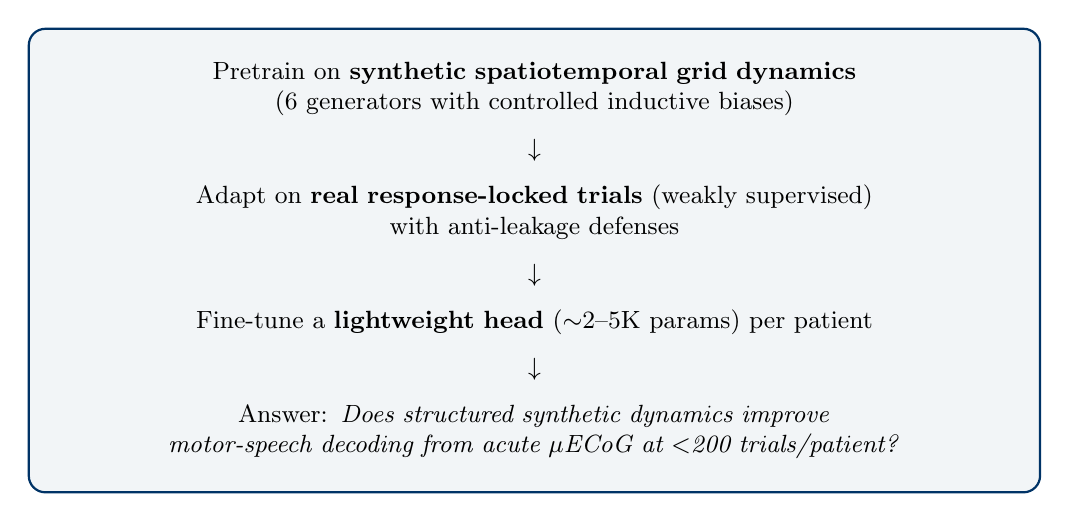
\begin{tikzpicture}
    \node[draw=DukeBlue, thick, rounded corners=6pt, fill=DukeBlue!5,
      text width=12cm, align=center, inner sep=12pt, font=\small] {
      Pretrain on \textbf{synthetic spatiotemporal grid dynamics}\\
      (6 generators with controlled inductive biases)\\[6pt]
      $\downarrow$\\[6pt]
      Adapt on \textbf{real response-locked trials} (weakly supervised)\\
      with anti-leakage defenses\\[6pt]
      $\downarrow$\\[6pt]
      Fine-tune a \textbf{lightweight head} ($\sim$2--5K params) per patient\\[6pt]
      $\downarrow$\\[6pt]
      Answer: \textit{Does structured synthetic dynamics improve}\\
      \textit{motor-speech decoding from acute \mcecog at $<$200 trials/patient?}
    };
  \end{tikzpicture}

  \vspace{0.8em}
  {\small 82 resolved decisions $\cdot$ 8 open questions $\cdot$ 7 first-round methods $\cdot$ 3 architecture families}
\end{center}
\vfill
\end{frame}

% ════════════════════════════════════════════════════════════
\appendix

\begin{frame}[noframenumbering]{Appendix: Priority Ablations}

\small
\begin{tabular}{@{}l L{10cm}@{}}
  \toprule
  \textbf{Ablation} & \textbf{Description} \\
  \midrule
  A. Pretext Objective & Masked spans (40--60\%) vs causal multi-step ($k$=1,3,5) vs varied span lengths \\
  B. Temporal Resolution & 20\,Hz (default) vs 40\,Hz. Lock early \\
  C. Patch Size & 1$\times$1 (default) vs 2$\times$2 vs conv stem \\
  D. Masking Ratio & 30\%, 50\%, 70\%. Interacts with temporal resolution \\
  \midrule
  \multicolumn{2}{@{}l}{\textbf{Tier 1} (gated on A\,$>$\,E)} \\
  \midrule
  E. Generator Family & Single-family runs from the ladder \\
  F. Freeze Level & Head+embed+LN vs head only vs full fine-tune \\
  G. Architecture Family & Full expansion of conv-GRU / bridge / ViT \\
  H. Spatial Pooling & Mean vs top-$k$ vs learned attention \\
  I. Source Weighting & Uniform vs similarity-weighted vs loss-balanced \\
  \bottomrule
\end{tabular}
\end{frame}

% ════════════════════════════════════════════════════════════

\begin{frame}[noframenumbering]{Appendix: Parameter Budgets}

\centering
\small
\renewcommand{\arraystretch}{1.1}
\begin{tabular}{@{}l r r r@{}}
  \toprule
  \textbf{Component} & \textbf{Conv-GRU} & \textbf{Bridge} & \textbf{ViT} \\
  \midrule
  Per-patient Conv2d       & 80 & 80 & --- \\
  Per-patient patch embed  & --- & --- & 256 \\
  Spatial projection       & --- & 576 + 256 & --- \\
  Encoder                  & 16,960 & 128 & 527,872 \\
  Predictor (BiGRU / Attn) & 37,632 & 37,632 & 395,520 \\
  Decoder (discarded)      & 16,640 & 65 & 129 \\
  Coord PE                 & --- & 256 & 512 \\
  CE head                  & 1,755 & 1,755 & 3,483 \\
  \midrule
  \textbf{Total pretrain}  & $\sim$71K & $\sim$39K & $\sim$927K \\
  \textbf{Stage 3 trainable} & $\sim$2.3K & $\sim$2.2K & $\sim$5.3K \\
  \bottomrule
\end{tabular}

\vspace{0.5em}
{\footnotesize All counts hand-computed---verify from prototype modules before running.}
\end{frame}

% ════════════════════════════════════════════════════════════

\begin{frame}[noframenumbering]{Appendix: Matching Statistics}

\small
\textbf{Computed for each generator vs real uECOG} (source patients only):

\vspace{0.3em}
\renewcommand{\arraystretch}{1.15}
\begin{tabular}{@{}L{3.5cm} L{9.5cm}@{}}
  \toprule
  \textbf{Statistic} & \textbf{Method} \\
  \midrule
  Temporal PSD & Welch (256-pt FFT, Hanning, 50\% overlap), concatenated across trials. Evoked + residual \\
  Spatial covariance & Exponential decay fit to Pearson $r$ vs distance (mm). Evoked + residual \\
  Amplitude distribution & Histogram of per-cell values; kurtosis + 95th percentile \\
  Dead-mask prevalence & Fraction of zero/inactive cells \\
  Event sparsity & Fraction of $|z| > 1.5$ cells per frame, per trial phase \\
  Phase structure & Trial-averaged spatial variance time series; peak/baseline ratio \\
  RT distribution & Mean, std, log-normal fit per patient \\
  \bottomrule
\end{tabular}

\vspace{0.5em}
\textbf{Coarse calibration}: 1--2 parameters/generator to land inside broad acceptable bands (PSD below 20\,Hz, spatial correlation 2--10 electrodes, kurtosis $>$ 2, event sparsity 5--30\%). Not optimization---prevents degenerate instantiation.
\end{frame}

% ════════════════════════════════════════════════════════════

\begin{frame}[noframenumbering]{Appendix: References}

\small
\begin{itemize}
  \item Lee, Han, Kumar, Agrawal (2026). ``Training Language Models via Neural Cellular Automata.'' arXiv:2603.10055
  \item Maes, Le Lidec, Scieur, LeCun, Balestriero (2026). ``LeWorldModel.'' arXiv:2603.19312
  \item Ghahramani \& Hinton (2000). ``Variational Learning for Switching State-Space Models.'' \textit{Neural Computation}
  \item Bertasius, Wang, Torresani (2021). ``Is Space-Time Attention All You Need?'' ICML 2021
  \item Tong et al.\ (2022). ``VideoMAE.'' NeurIPS 2022
  \item Assran et al.\ (2023). ``I-JEPA.'' CVPR 2023
  \item Spalding et al.\ (2025). Cross-patient speech decoding from uECOG
  \item Singh et al.\ (2025). Per-patient layers + frozen shared backbone
  \item Duraivel et al.\ (2023). Micro-ECoG spatial resolution
  \item Duraivel et al.\ (2025). Pseudo-word repetition, overlapping patients
\end{itemize}
\end{frame}

\end{document}
